\documentclass{article}

\usepackage{tikz-qtree}
\tikzset{ n/.style={draw=none} }

\title{Assignment 4: Binary Trees}
\author{Harrison Maksimik}
\date{2023/11/26}

\begin{document}

\maketitle
\begin{enumerate}
\item
  Draw an expression tree corresponding to each of the following
  
  \begin{enumerate}
  \item
    Inorder traversal is: x / y + 3 * b / c
    
    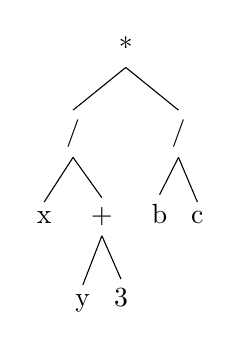
\begin{tikzpicture}
      \Tree [.* [./ x [.+ y 3 ] ] [./ b c ] ]
    \end{tikzpicture}
  \item
    Postorder traversal is: x y z + a b – c * / –

    \begin{tikzpicture}
      \Tree [.– x [./ [.+ y z ] [.* [.– a b ] c ] ] ]
    \end{tikzpicture}
  \item
    Preorder traversal is: * + a – x y / c d

    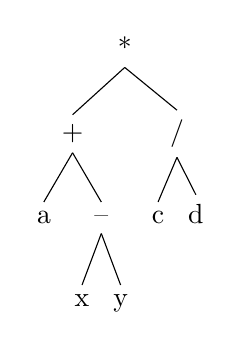
\begin{tikzpicture}
      \Tree [.* [.+ a [.– x y ] ] [./ c d ] ]
    \end{tikzpicture}
  \end{enumerate}
\item
  Considered the output of a \texttt{to\_string} method below and show the tree that would be built by the following data lines is the binary search tree

  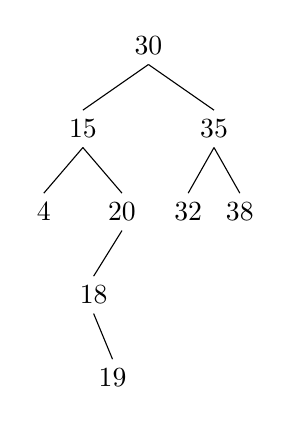
\begin{tikzpicture}
    \Tree [.30 [.15 4 [.20 [.18 \edge[n];[.{} ] 19 ] \edge[n];[.{} ] ] ] [.35 32 38 ] ]
  \end{tikzpicture}
\end{enumerate}

\end{document}
